\section{To-do List Functionalities guide}
\begin{figure}[H]
	\centering
	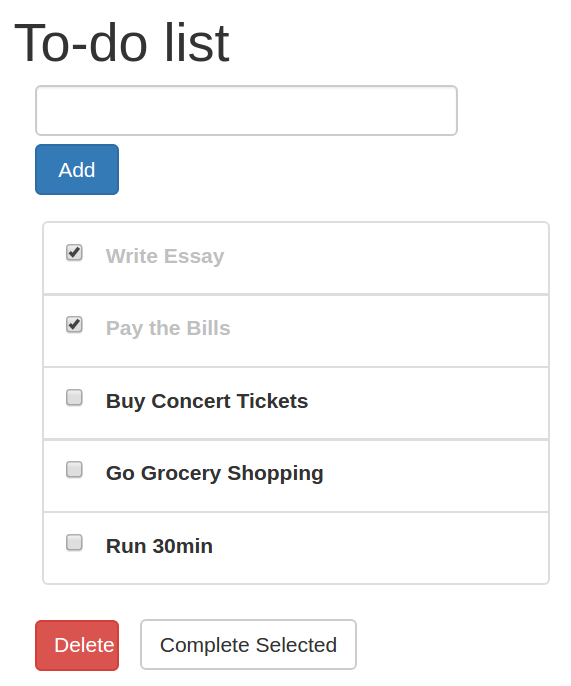
\includegraphics[width=7cm]{../../documenti/UserManualDemo/demo_screens/todo.png}
	\caption{To-do List}
\end{figure}
\subsection{Adding an Item to the List}
Type the text of the entry you wish to add and click ``Submit''. The new item will appear on the list.
\subsection{Mark Items as completed}
Select the entries you wish to complete and click on ``Complete Selected'' to mark them as completed. 
\subsection{Removing Items From the List}
Select the entries you wish to remove and click on ``Delete Selected'' to remove them from the list.

\section{\DemoName{} Functionalities guide}
\subsection{Customer}
\subsubsection{Consulting the Menu}
\begin{figure}[H]
	\centering
	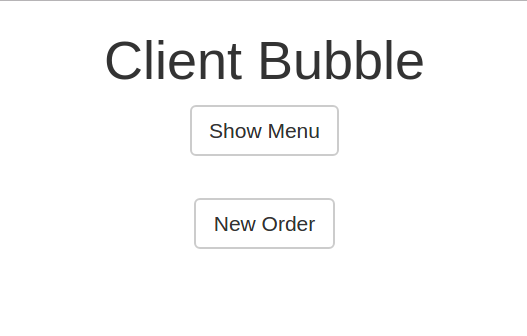
\includegraphics[width=7cm]{../../documenti/UserManualDemo/demo_screens/client_main.png}
	\caption{Customer Main Page}
\end{figure}
\paragraph{Customer Main Page}
In the Customer Main Page it is possible to access the menu by clicking the button labeled as ``Menu''.
\begin{figure}[H]
	\centering
	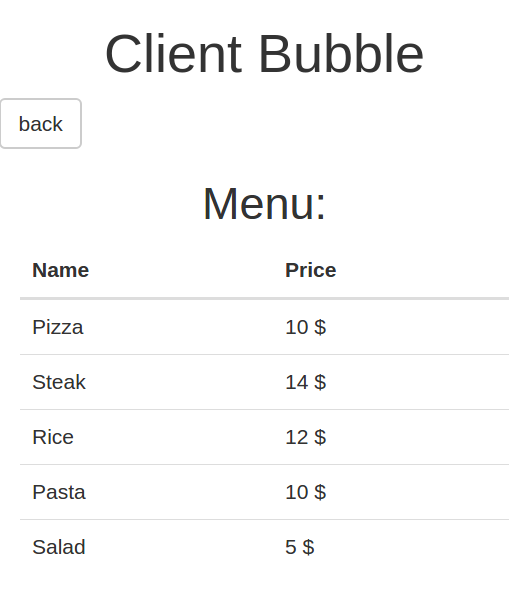
\includegraphics[width=7cm]{../../documenti/UserManualDemo/demo_screens/client_menu.png}
	\caption{Customer Menu Page}
\end{figure}
\paragraph{Menu Page }
In the Menu Page it is possible for the Customer to consult the Menu presenting all the dishes available to order in the restaurant.
By clicking on the ``Back'' button the Customer will be redirected to the Customer main page.

\subsubsection{Placing an Order}
\begin{figure}[H]
	\centering
	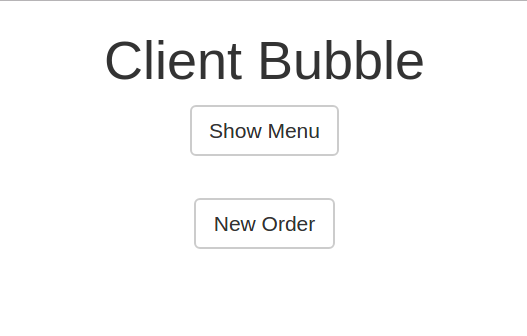
\includegraphics[width=7cm]{../../documenti/UserManualDemo/demo_screens/client_main.png}
	\caption{Customer Main Page}
\end{figure}
\paragraph{Customer Main Page}
In the Customer Main Page it is possible to access the Order page by clicking on the ``Make a new Order'' button.
\begin{figure}[H]
	\centering
	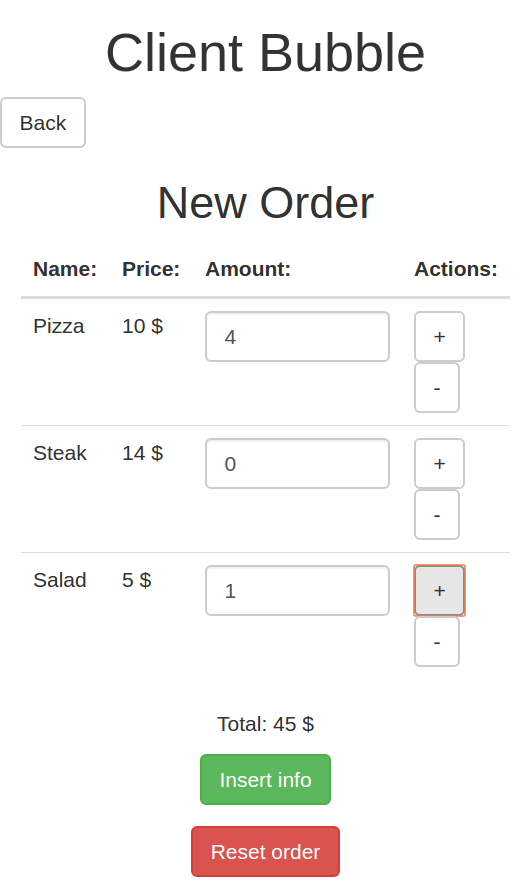
\includegraphics[width=7cm]{../../documenti/UserManualDemo/demo_screens/client_dishes.png}
	\caption{Customer Order Page}
\end{figure}
\paragraph{New Order Page}
New Order Page shows all the available dishes and allows the Customer to set the quantities of each dish, either by inserting a number or by increasing and decreasing them through the specific buttons marked by the plus and minus symbols. The page also shows the total amount due for the order.
By clicking on Reset Order the quantities for all the dishes will be reset to zero.
To continue the order procedure a Customer must click ``Insert Info''. 
It is possible for a Customer to go back to the main page by clicking ``Back''.

\begin{figure}[H]
	\centering
	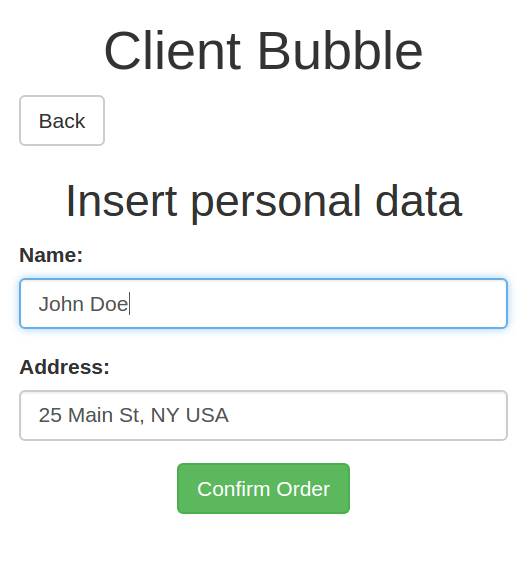
\includegraphics[width=7cm]{../../documenti/UserManualDemo/demo_screens/client_info.png}
	\caption{Customer's Info Page}
\end{figure}
\paragraph{Insert Personal Data}
In this page it is possible for the Customer to fill in a form by typing a Name and an Address to have its order be delivered at the specified location. To confirm the order a Customer must click on 'confirm order'. 
It's possible for a Customer to go back to the order page by clicking 'back'.

\begin{figure}[H]
	\centering
	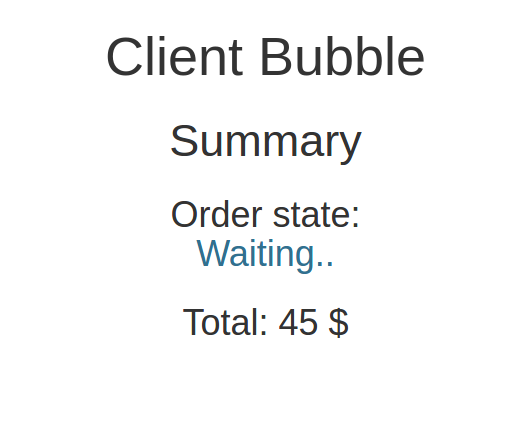
\includegraphics[width=7cm]{../../documenti/UserManualDemo/demo_screens/client_summary.png}
	\caption{Customer Summary Page}
\end{figure}
\paragraph{Summary or Waiting Page}
After an order has been placed the user is redirected to the summary/waiting page where a summary of the order is shown and the Customer is advised to wait until the dishes are ready.

\begin{figure}[H]
	\centering
	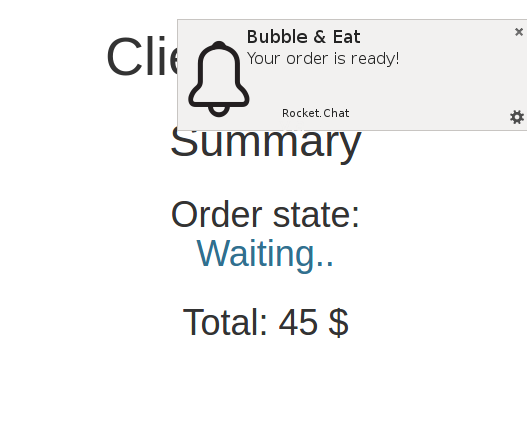
\includegraphics[width=7cm]{../../documenti/UserManualDemo/demo_screens/client_notification.png}
	\caption{Customer Notification Page}
\end{figure}
\paragraph{Notification}
When the order is marked as completed by the Chef, a notification is sent to warn the Customer that its meal is ready.

\subsection{Chef}
\subsubsection{Consulting the Orders}
\begin{figure}[H]
	\centering
	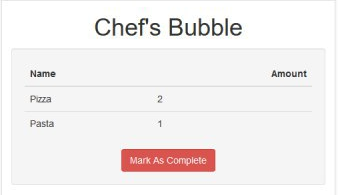
\includegraphics[width=7cm]{../../documenti/UserManualDemo/demo_screens/chef_orders.png}
	\caption{Chef Main Page}
\end{figure}
In the Chef order page it is possible to view all the orders and mark them as completed.

\begin{figure}[H]
	\centering
	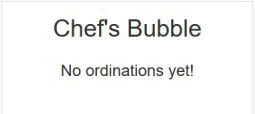
\includegraphics[width=7cm]{../../documenti/UserManualDemo/demo_screens/chef_none.png}
	\caption{Chef No Orders}
\end{figure}
The Chef will be informed if there isn't any order yet.

\begin{figure}[H]
	\centering
	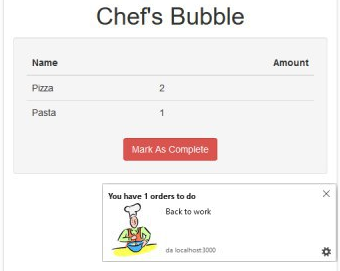
\includegraphics[width=7cm]{../../documenti/UserManualDemo/demo_screens/chef_notification.png}
	\caption{Chef Notification}
\end{figure}
The Chef will be alerted whith a notification when a new order is placed.

\subsection{Manager}
\subsubsection{Accessing the Menu Operations}
\begin{figure}[H]
	\centering
	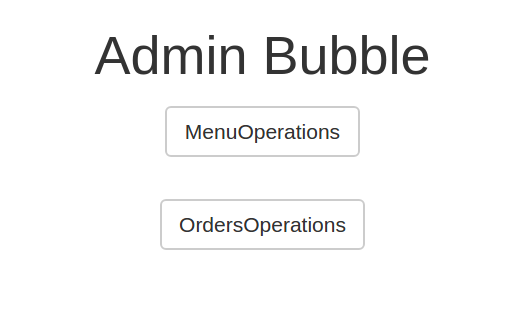
\includegraphics[width=7cm]{../../documenti/UserManualDemo/demo_screens/admin_main.png}
	\caption{Manager Main Page}
\end{figure}
\paragraph{Manager Main Page}
In the Manager main page it is possible to access the Menu Operations page by clicking the button labeled as ``Menu Operations''.

\begin{figure}[H]
	\centering
	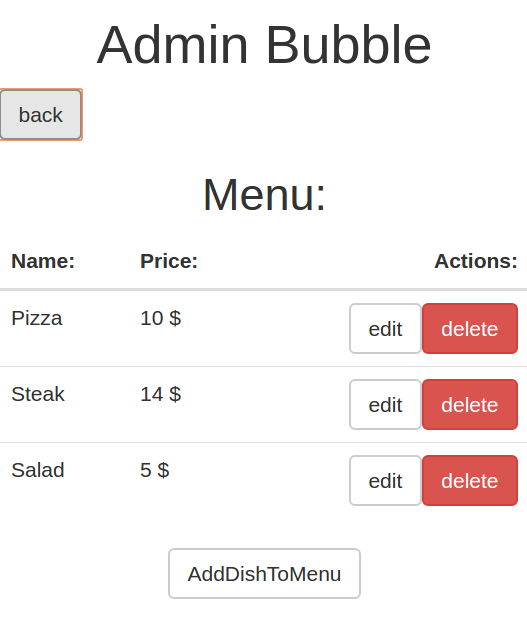
\includegraphics[width=7cm]{../../documenti/UserManualDemo/demo_screens/admin_menu.png}
	\caption{Manager Menu Page}
\end{figure}
\paragraph{Menu Operations}
In the menu operations page it is possible for the Manager to decide whether to add, edit or delete the different dishes.
By clicking ``Delete'' on a certain dish, it will be deleted from the restaurant's menu.
By clicking ``Edit'' on a certain dish, the Manager will be redirected to the Edit Dish page where it will be possible to Edit the selected dish.
By clicking ``Add'' the Manager will be redirected to Add Dish Page.
It's possible for the manager to go back to the main page by clicking 'back'.

\begin{figure}[H]
	\centering
	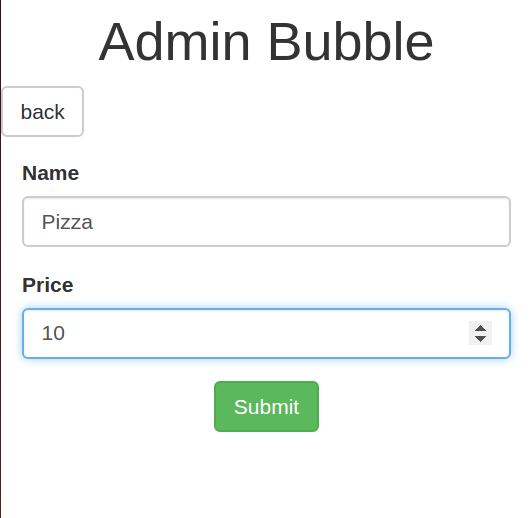
\includegraphics[width=7cm]{../../documenti/UserManualDemo/demo_screens/admin_edit.png}
	\caption{Manager Edit dish Page}
\end{figure}
\paragraph{Edit Dish Page}
In the edit dish page a form is shown containing the dish's current name and price that can be edited and saved by clicking ``Submit''.
It is possible for the Manager to go back to the Menu Operation Page by clicking 'back'.

\begin{figure}[H]
	\centering
	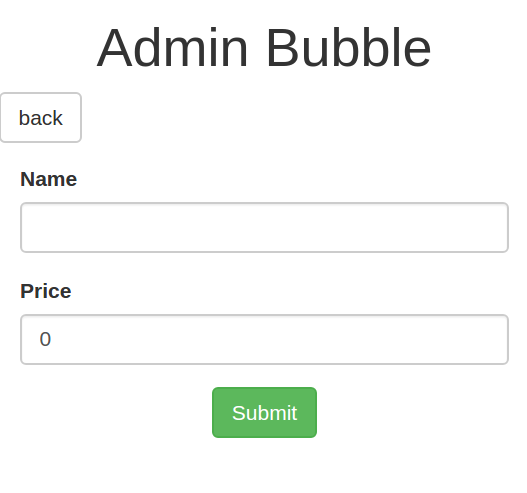
\includegraphics[width=7cm]{../../documenti/UserManualDemo/demo_screens/admin_add.png}
	\caption{Manager Add dish Page}
\end{figure}
\paragraph{Add Dish Page}
In the Add Dish Page a form is shown with an empty text input for the new dish's Name and a Price input where the price of the new dish can either be typed or increased and deacresed through the specific buttons. The new dish can be added by clicking ``Submit''.
It's possible for the manager to go back to the Menu Operation page by clicking ``Back''.

\subsubsection{Accessing the Orders Operations}
\begin{figure}[H]
	\centering
	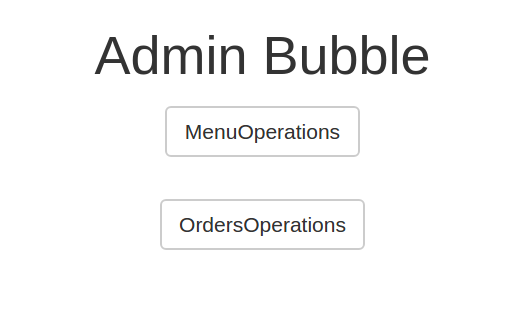
\includegraphics[width=7cm]{../../documenti/UserManualDemo/demo_screens/admin_main.png}
	\caption{Manager Main Page}
\end{figure}
\paragraph{Manager Main Page}
In the Manager Main Page it is possible to access the Orders Operations page by clicking the button labeled as ``Orders Operations''.

\begin{figure}[H]
	\centering
	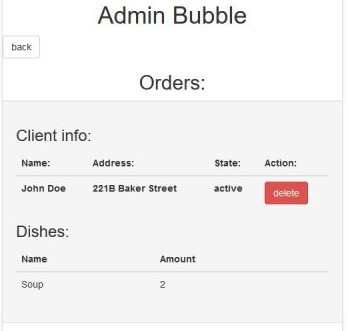
\includegraphics[width=7cm]{../../documenti/UserManualDemo/demo_screens/admin_orders.png}
	\caption{Manager Orders Operations}
\end{figure}
\paragraph{Manager Orders Operations}
In the Manager's Orders Operations page it is possible for the Manager to see all the orders placed by the customers, in this page the Manager is also able to delete these orders.
It is possible for the Manager to go back to the Orders Operation Page by clicking 'back'.



